% Messwerte: Alle gemessenen Größen tabellarisch darstellen
% Auswertung: Berechnung geforderter Ergebnisse mit Schritten/Fehlerformeln/Erläuterung/Grafik (Programme)
\section{Auswertung}
\label{sec:auswertung}

Der Innenwiderstand des Funktionsgenerators ist mit $R_0 = \qty{600}{\ohm}$ angegeben, während sich der
Wert für den RC\hspace{0.15ex}-Kreis zu $R = \qty{11}{\kilo\ohm}$ bemisst. Mit $\,\tilde{\!R} = R_0 + R$
ist daher eine weitere Relation zu berücksichtigen. Ausgleichsrechnungen werden
mit den Bibliotheken NumPy \cite{numpy} und SciPy \cite{scipy} unter Python \cite{python} durchgeführt. Zum
Erstellen von Grafiken wird Matplotlib \cite{matplotlib} verwendet.

\subsection{Entladungskurve}

\begin{figure}[H]
	\includegraphics{build/t-U_plot.pdf}
	\caption{Messdaten mit linearisierter Regressionsrechnung.}
	\label{fig:entladung}
\end{figure}

Der exponentielle Verlauf der Daten in Tabelle \ref{tab:entladung} kann mit
$U_0 = \input{build/t-U_0.tex}$ in die Form
\begin{equation}
	\ln \pfrac{U}{U_{\! 0}} = v t + w
\end{equation}
gebracht werden, sodass sich nach \eqref{eqn:regression} mittels \verb+numpy.polyfit+ die in Abbildung
\ref{fig:entladung} gezeigte optimale Ausgleichsgerade ermitteln lässt. Die fehlerbehafteten Parameter
\begin{align*}
	v = \input{build/t-U_v.tex} && w = \input{build/t-U_w.tex}
\end{align*}
folgen aus der automatisch generierten Kovarianzmatrix, indem die Quadratwurzeln der Diagonalelemente
berechnet werden. Der Wert $RC = -v^{-1} = \input{build/t-U_RC.tex}$ ergibt sich somit als Maß
der Zeitkonstante. 

\begin{table}
	\centering
	\caption{Abgelesene Daten aus dem zeitlichen Verlauf der Entladung.}
	\input{build/t-U_table.tex}
	\label{tab:entladung}
\end{table}

\subsection{Übertragungsfunktion}

\begin{figure}[H]
	\includegraphics{build/f-U_plot.pdf}
	\caption{Messdaten mit nichtlinearer Näherungsrechnung.}
	\label{fig:übertragung}
\end{figure}
Für den frequenzabhängigen Amplitudenverlauf \eqref{eqn:amplitude_frequenz} wird
\verb+scipy.optimize.curve_fit+ als generalisierte Alternative zum vorherigen Vorgehen mit
$U_0 = \input{build/f-U_0.tex}$ genutzt. Zu den Werten aus Tabelle \ref{tab:übertragung} ergibt
sich so der Verlauf in Abbildung \ref{fig:übertragung} sowie der Parameter
$\,\tilde{\!R}C = \input{build/f-U_RC.tex}$. Die Korrektur für den Innenwiderstand $R_0$ lautet
\begin{equation*}
	R = \pfrac{11}{\num{11.6}} \,\tilde{\!R}
\end{equation*}
und liefert dann die Zeitkonstante $RC = \input{build/f-U_RC_corr.tex}$.

\begin{table}
	\centering
	\caption{Aufgenommene Messdaten unter Variation der Frequenz.}
	\input{build/f-U_table.tex}
	\label{tab:übertragung}
\end{table}

\subsection{Phasenverlauf}

\begin{figure}[H]
	\includegraphics{build/f-phi_plot.pdf}
	\caption{Messdaten mit nichtlinearer Näherungsrechnung.}
	\label{fig:phase}
\end{figure}
\begin{figure}[H]
	\includegraphics{build/polar_plot.pdf}
	\caption{Theoriekurve mit Messwerten.}
	\label{fig:polar}
\end{figure}

Die Messwerte in Tabelle \ref{tab:phase} werden zunächst für Phasensprünge korrigiert. Unter analoger
Anwendung von \verb+scipy.optimize.curve_fit+ folgen daraus die \mbox{Regressionskurve \eqref{eqn:phase}
in} Abbildung \ref{fig:phase} mit dem charakteristischen Parameter $\,\tilde{\!R}C = \input{build/f-phi_RC.tex}$
sowie der korrigierte Wert $RC = \input{build/f-phi_RC_corr.tex}$ als Zeitkonstante. Abbildung \ref{fig:polar}
stellt dann noch den phasenbedingten Amplitudenverlauf nach Vorschrift \eqref{eqn:amplitude_phase} dar.

\begin{table}
	\centering
	\vspace{2.46ex}
	\caption{Aufgenommene Messdaten unter Variation der Frequenz.}
	\input{build/f-phi_table.tex}
	\label{tab:phase}
\end{table}

\subsection{Integration}

\begin{figure}
	\begin{subfigure}{0.32\textwidth}
		\centering
		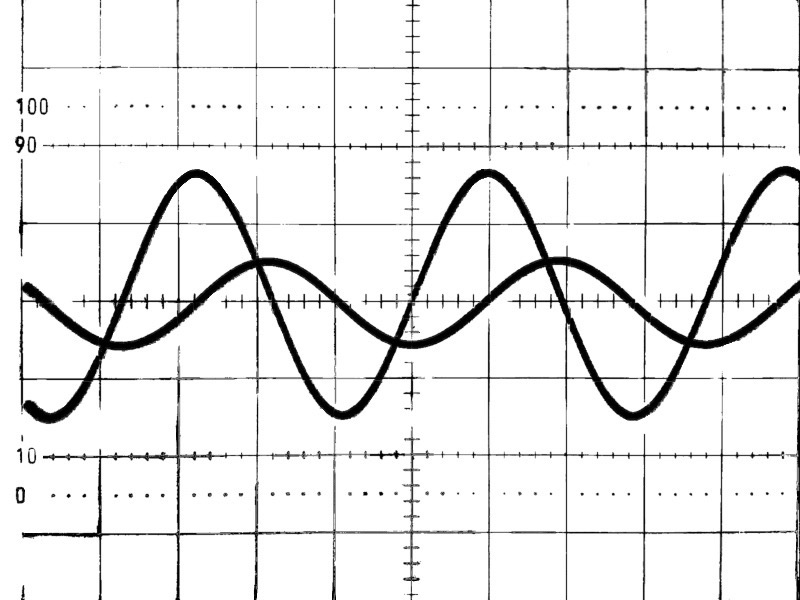
\includegraphics[height=3.5cm]{content/sinus.jpg}
		\caption{Sinusspannung}
	\end{subfigure}
	\hfill
	\begin{subfigure}{0.32\textwidth}
		\centering
		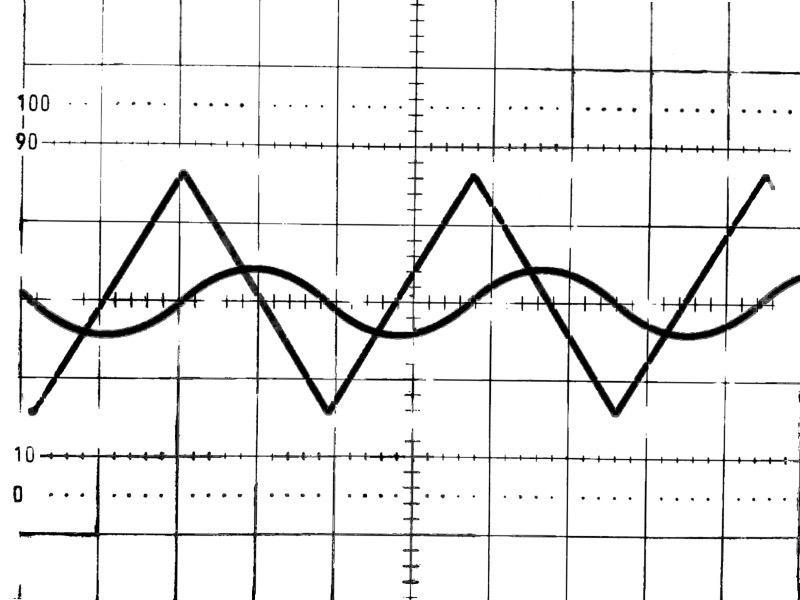
\includegraphics[height=3.5cm]{content/dreieck.jpg}
		\caption{Dreiecksspannung}
	\end{subfigure}
	\hfill
	\begin{subfigure}{0.32\textwidth}
		\centering
		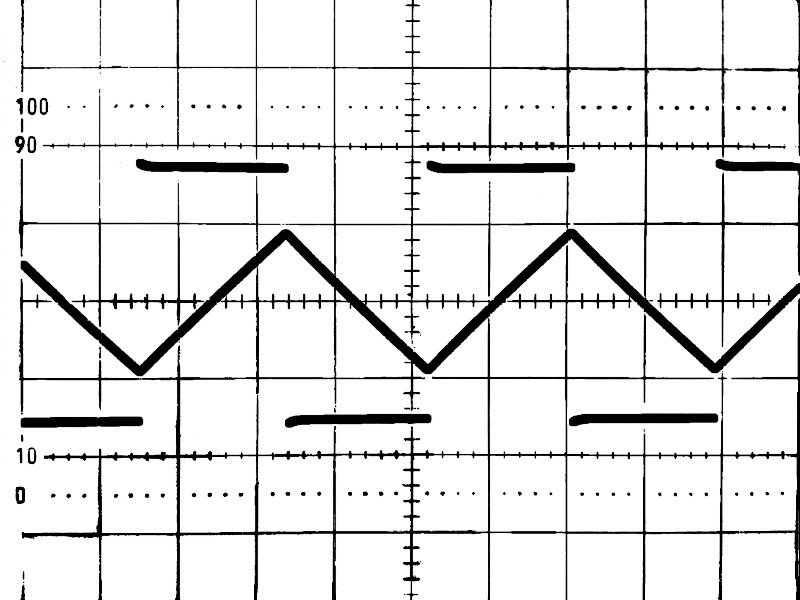
\includegraphics[height=3.5cm]{content/rechteck.jpg}
		\caption{Rechtecksspannung}
	\end{subfigure}
	\caption{Integration verschiedener Eingangssignale am RC\hspace{0.15ex}-Glied.}
	\label{fig:integral}
\end{figure}

Anhand der Spannungsverläufe in Abbildung \ref{fig:integral} lässt sich exemplarisch die Anwendung als
Integrationsglied nach \eqref{eqn:integral} erkennen. Angelegt ist dazu eine Frequenz von
$\nu = \qty{10}{\kilo\hertz}$.
